\RequirePackage{fix-cm}
\documentclass[twocolumn]{svjour3}
\smartqed
\usepackage{graphicx}
\graphicspath{{figures/}}
\tolerance=1
\emergencystretch=\maxdimen
\hyphenpenalty=10000
\hbadness=10000
\def\makeheadbox{\relax}
\usepackage[numbers]{natbib}
\usepackage{algorithm}
\usepackage{algpseudocode}
\renewcommand{\algorithmicrequire}{\textbf{Input:}}
\renewcommand{\algorithmicensure}{\textbf{Output:}}
\usepackage{amsmath,amssymb}
\usepackage{tabularx}
\usepackage{booktabs}
\usepackage{url}
\usepackage{tikz}
\usetikzlibrary{arrows.meta, positioning, shapes.geometric}
\usepackage[dvipsnames,table]{xcolor}
\usepackage{microtype}
\usepackage[most]{tcolorbox}
\newtcolorbox{keyresult}{
  enhanced,
  breakable,
  colback=blue!3!white,
  boxrule=0pt,
  frame hidden,
  borderline west={3pt}{0pt}{blue!45!black!65},
  left=8pt, right=5pt, top=4pt, bottom=4pt,
  before skip=\medskipamount,
  after skip=\medskipamount,
  sharp corners,
}
\usepackage{latexsym}
\usepackage{enumitem}
\usepackage{mathptmx}
\usepackage{pgfplots}
\pgfplotsset{compat=1.12}
\usepackage{float}
\usepackage{stfloats}

\begin{document}

\title{StatefulAutoscaler: A Connection-Aware Kubernetes Controller for
Persistent-Connection Workloads --- Design, Validation, and Protocol
Generalization}

\titlerunning{StatefulAutoscaler: Connection-Aware Kubernetes Autoscaling}

\author{
Abhash Behera \and
Aditya Hota \and
Suprit Kumar Naik \and
Ritesh Kumar Singh
}

\authorrunning{ }

\date{Received: -; Accepted: -}

\institute{
\textbf{Abhash Behera} \at
Department of Computer Science and Engineering, \\
C V Raman Global University, Bhubaneswar 752054, India \\
\email{abhasbehera320@gmail.com}
\and
\textbf{Aditya Hota} \at
Department of Computer Science and Engineering, \\
C V Raman Global University, Bhubaneswar 752054, India \\
\email{adityahota99@gmail.com}
\and
\textbf{Suprit Kumar Naik} \at
Department of Computer Science and Engineering, \\
C V Raman Global University, Bhubaneswar 752054, India \\
\email{supritkumarnaik17@gmail.com}
\and
\textbf{Ritesh Kumar Singh} \at
Department of Computer Science and Engineering, \\
C V Raman Global University, Bhubaneswar 752054, India \\
\email{rihankumar2004@gmail.com}
}

\maketitle

\begin{abstract}
CPU-based Kubernetes HPA is empirically demonstrated in the companion paper~\cite{behera2026hpa}
to exhibit three structural failure modes for stateful WebSocket workloads: 87.5\%
over-provisioning, reconnection storms reaching 1,400~connections/second, and permanent
staircase connection destruction. This paper presents the design, implementation, and
multi-baseline experimental validation of the \texttt{StatefulAutoscaler} --- a custom Kubernetes
controller built on the Kubebuilder SDK~\cite{kubebuilder_docs} that resolves all three failure
modes by scaling exclusively on \texttt{sum(active\_connections)} queried from Prometheus and
incorporating a sliding-window stabilization mechanism (\texttt{scaleDownCooldownSeconds}) to
suppress premature scale-down during transient connection drops. Controlled experimental
evaluation across a two-cycle reconnection storm simulation (Experiment~C, five independent
runs) demonstrates exact replica targeting ($\lceil800/100\rceil = 8$ replicas, 0\% waste), zero
connection loss across all observed scaling events, and complete pod preservation through a
90-second disconnection gap via the stabilization window (scale-down reaction time
$119 \pm 2$~s; pod-seconds $4{,}280 \pm 67$). Comparative baseline evaluation against HPA
augmented with a custom connection-count metric via the Prometheus Adapter (Experiment~D,
five runs) and KEDA configured with a matching \texttt{cooldownPeriod} (Experiment~E, five
runs) reveals a nuanced finding: all three connection-aware configurations preserve pods
through the 90-second DROP~1 gap, with the \texttt{StatefulAutoscaler} differentiating on
scale-up latency (22~s vs.\ 26~s for KEDA and 54~s for HPA+custom metric) and final scale-down efficiency (119~s vs.\ 313~s for Experiment~D). Three adversarial failure scenarios establish the operational envelope: metric staleness
degrades gracefully to a reaction lag bounded by the scrape interval; instantaneous connection
spikes expose pod scheduling latency as the binding constraint; Prometheus unavailability
triggers safe-default hold behavior with no connection loss. MQTT generalization experiments
confirm protocol-agnosticism: the identical controller binary, with zero source-code changes,
scales 44\% faster than CPU HPA (38~s vs.\ 68~s), preserves all 339~sessions during a forced
scale-down (maximum step-drop: 2 vs.\ 639-connection cliff), and redistributes sessions across
pods via drain-reconnect semantics.

\keywords{Kubernetes \and Custom Controller \and StatefulAutoscaler \and WebSocket \and
MQTT \and Connection-Aware Autoscaling \and Prometheus \and Sliding-Window
Stabilization \and KEDA \and Kubebuilder \and Reconnection Storm}
\end{abstract}



%% ============================================================
\section{Introduction}
\label{sec:intro}
%% ============================================================

The failure of CPU-based Kubernetes Horizontal Pod Autoscaler (HPA)~\cite{k8s_hpa_docs} for stateful
persistent-connection workloads is established in the companion paper~\cite{behera2026hpa}.
Three failure modes are documented and quantified: over-provisioning by 87.5\% under cyclic
load (15 replicas vs.\ the correct 8, with \texttt{maxReplicas} exhausted within 99~seconds);
reconnection storms reaching 1,400~connections/second triggered directly by HPA scale-down
events; and permanent staircase connection destruction that reduced an 800-session population
to 79 with zero recovery. That paper establishes that these failure modes are
\textit{architectural}, not configurational: they arise from the structural mismatch between CPU
utilization as a scaling signal and the actual workload state that must be protected (active
connection sessions), and cannot be remediated by HPA parameter tuning alone.

This mismatch identifies a concrete design gap. No existing Kubernetes-native mechanism
simultaneously provides (a)~a connection-count scaling signal that faithfully encodes workload
state, and (b)~connection-context-aware stabilization semantics that suppress premature
scale-down while live sessions are present. The Prometheus Adapter~\cite{prometheus_adapter}
can supply the signal but cannot alter HPA's built-in stabilization logic, which stabilizes
CPU-derived replica recommendations rather than connection-derived capacity requirements.
KEDA~\cite{keda_docs} provides event-driven scaling via a configurable cooldown period but
delegates all pod termination decisions to HPA without per-cycle step-size bounding, and
exposes no mechanism to limit the blast radius of a single scale-down event in terms of
connections destroyed.

This paper addresses both gaps through the design, implementation, and multi-baseline
experimental validation of the \textbf{\texttt{StatefulAutoscaler}} --- a custom Kubernetes
controller built with the Kubebuilder~\cite{kubebuilder_docs} SDK. The controller owns both
the metric selection (\texttt{sum(active\_connections)} from Prometheus; CPU is never
consulted) and the scale-down lifecycle (a sliding-window high-water-mark stabilization
mechanism that retains the memory of recent connection demand). This paper makes the
following contributions:

\begin{enumerate}[leftmargin=*]
\item \textbf{Complete design and implementation of the \texttt{StatefulAutoscaler}.}
  We present the CRD specification, reconciliation algorithm (Algorithm~\ref{alg:reconcile}),
  and sliding-window stabilization mechanism, with formal analysis of stability properties,
  convergence bounds (Equation~\ref{eq:convergence}), and oscillation conditions.

\item \textbf{Controlled experimental validation with statistical replication (Experiment~C).}
  Under a two-cycle reconnection storm simulation with five independent runs, we
  demonstrate exact replica targeting ($\lceil800/100\rceil = 8$, versus CPU HPA's~15),
  complete pod preservation through a 90-second total disconnection gap, and zero
  connection loss across all scaling events. Statistical reproducibility is confirmed
  (scale-down reaction $\sigma = 2$~s, pod-seconds $\sigma = 67$).

\item \textbf{Comparative baseline evaluation (Experiments D and E).} To determine
  whether performance differences arise from metric choice alone or controller architecture,
  we evaluate HPA augmented with a custom connection-count metric (Experiment~D, five
  runs) and KEDA with a matched \texttt{cooldownPeriod} (Experiment~E, five runs) under
  identical workloads. Both baseline configurations preserve pods through DROP~1,
  establishing nuanced differentiators: scale-up latency ($22$~s vs.\ $54$~s vs.\ $26$~s) and
  final scale-down efficiency ($119$~s vs.\ $313$~s).

\item \textbf{Adversarial failure scenario characterization.} Three adversarial
  conditions --- metric staleness under extended scrape intervals, instantaneous connection
  spikes with no ramp stagger, and Prometheus unavailability during active load --- bound
  the operational envelope of the controller with measured reaction times, connection
  overshoot statistics, and explicit boundary conditions.

\item \textbf{Protocol generalization validation on MQTT.} Using the identical controller
  binary with zero source-code changes, we resolve all three MQTT-specific HPA failure
  modes (scale-up blindness, session pinning, destructive scale-down) and demonstrate
  44\% faster scale-up than CPU HPA, zero sessions destroyed during forced scale-down
  (maximum step-drop: 2 vs.\ a 639-connection cliff), and drain-based session redistribution.
\end{enumerate}

The remainder of this paper is structured as follows. Section~\ref{sec:related} surveys related
work. Section~\ref{sec:background} provides background on the HPA control architecture and
the failure characterization this paper builds upon. Section~\ref{sec:controller} details the
design and implementation of the \texttt{StatefulAutoscaler}. Section~\ref{sec:evaluation}
presents Experiment~C validation results. Section~\ref{sec:baselines} presents baseline
comparisons against HPA with custom metrics (Experiment~D) and KEDA (Experiment~E).
Section~\ref{sec:failure_analysis} characterizes adversarial failure conditions.
Section~\ref{sec:discussion} analyzes implications. Section~\ref{sec:mqtt_extension} presents
the MQTT protocol generalization experiments. Section~\ref{sec:limitations} discusses
limitations. Section~\ref{sec:future_work} outlines future directions. Section~\ref{sec:conclusion}
concludes.



%% ============================================================
\section{Related Work}
\label{sec:related}
%% ============================================================

\subsection{Kubernetes HPA with Custom Metrics}

Kubernetes supports application-defined scaling signals through the Prometheus
Adapter~\cite{prometheus_adapter}, enabling HPA to react to metrics beyond CPU ---
including HTTP request rate, queue depth, and custom application counters. Qu et
al.~\cite{qu2018auto} surveyed HTTP-rate-based autoscaling strategies; Rossi et
al.~\cite{rossi2020horizontal} studied hybrid CPU-and-traffic approaches. However, all these
formulations presuppose that the scaling metric is stateless across pod boundaries --- an
assumption violated by connection-holding protocols where session state is affined to a
specific pod. Crucially, even when HPA is correctly configured with a connection-count custom
metric via the Prometheus Adapter, metric choice alone is insufficient: without
connection-lifecycle-aware scale-down policies, HPA will still scale down during transient
connection dropout gaps, destroying the session state it should protect. This is empirically
demonstrated in Experiment~D (Section~\ref{sec:experiment_d}).

\subsection{Event-Driven Autoscaling: KEDA}

Kubernetes Event-Driven Autoscaling (KEDA)~\cite{keda_docs} extends HPA by watching
external metrics --- including Prometheus gauges such as \texttt{active\_connections} --- and
drives replica counts by managing the \texttt{spec.minReplicas} field of an underlying HPA
object. Scale-up proceeds by raising this floor; scale-down by lowering it, after which HPA
executes the actual pod termination. This delegation creates two structural limitations for
stateful WebSocket workloads. First, KEDA does not expose a per-cycle
\texttt{maxScaleDownStep} parameter: once \texttt{minReplicas} is lowered, HPA may remove
many pods in a single reconciliation step with no application-level bound on the scale of that
event. Second, neither KEDA nor HPA has awareness of the OS-level termination window:
when Kubernetes kills a pod, the operating system requires approximately 30~seconds to
propagate TCP RST packets to connected clients. A configurable \texttt{cooldownPeriod} in
KEDA can delay scale-down after a metric drop. Experiment~E (Section~\ref{sec:experiment_e})
directly tests KEDA with a matched 120-second \texttt{cooldownPeriod}, confirming that it
successfully holds pods through the 90-second DROP~1 gap; the architectural distinction
relative to the \texttt{StatefulAutoscaler} manifests in convergence profile and the absence of
per-cycle step-rate bounding.

\subsection{Stateful Workloads and Protocol-Aware Autoscaling}

Dickel et al.~\cite{dickel2019stateful} identified stateful autoscaling as an open research
challenge specific to IoT gateway deployments using WebSocket and MQTT. While their work
motivates the need for protocol-aware scaling and proposes monitoring active connections via
Prometheus, it neither provides a quantitative characterization of HPA failure modes nor
implements or validates a complete controller-level solution. The companion
paper~\cite{behera2026hpa} fills the characterization gap; this paper fills the solution gap.

\subsection{Machine Learning and Predictive Autoscaling}

Reinforcement learning approaches~\cite{rossi2020horizontal,imdoukh2020machine} and
machine learning-based workload prediction~\cite{toka2021machine,zhong2020machine} have
been proposed to improve autoscaling responsiveness. While these approaches offer proactive
scaling capability, they introduce model training complexity and workload-specific data
requirements. More importantly, they do not address the structural problem of
connection-state destruction during scale-down, which persists regardless of \textit{when}
scaling decisions are made; the issue is \textit{whether} a scale-down decision is made while
live connections are present, not how accurately the decision is timed.

\subsection{Custom Kubernetes Controllers}

The Kubebuilder SDK~\cite{kubebuilder_docs} provides a framework for implementing
Custom Resource Definition (CRD)-based Kubernetes controllers using the
\texttt{controller-runtime} library. The CRD pattern is the standard Kubernetes extension
mechanism for domain-specific control loops, and enables operators to define new API types
with declarative specifications and reconciliation-loop logic without modifying the core
Kubernetes API server.

\subsection{MQTT Autoscaling}

MQTT~\cite{mqtt_v31} maintains long-lived TCP sessions with low CPU activity during idle
periods, exhibiting the same signal mismatch as WebSocket for CPU-based HPA~\cite{soni2017mqtt}.
The companion paper~\cite{behera2026hpa} documents three MQTT-specific HPA failure modes
qualitatively; this paper provides experimental validation that the \texttt{StatefulAutoscaler}
resolves all three using an unmodified controller binary.

\subsection{Research Gap}

To the best of our knowledge, no prior work has simultaneously: (i)~designed, implemented,
and validated a connection-aware Kubernetes controller with sliding-window stabilization
semantics explicitly targeting reconnection storm resilience; (ii)~compared four distinct scaler
configurations (CPU HPA, custom-metric HPA, KEDA, and a custom controller) under
identical WebSocket workloads with five-run statistical replication; and (iii)~validated the same
controller binary on a second persistent-connection protocol (MQTT) with drain-reconnect
session redistribution semantics. This paper addresses all three dimensions.



%% ============================================================
\section{Background}
\label{sec:background}
%% ============================================================

This section provides the context needed for a reader who has not read the companion
paper~\cite{behera2026hpa}. Full pipeline characterization and behavioral baselines for
stateless HTTP workloads are documented there.

\begin{figure*}[t]
\centering
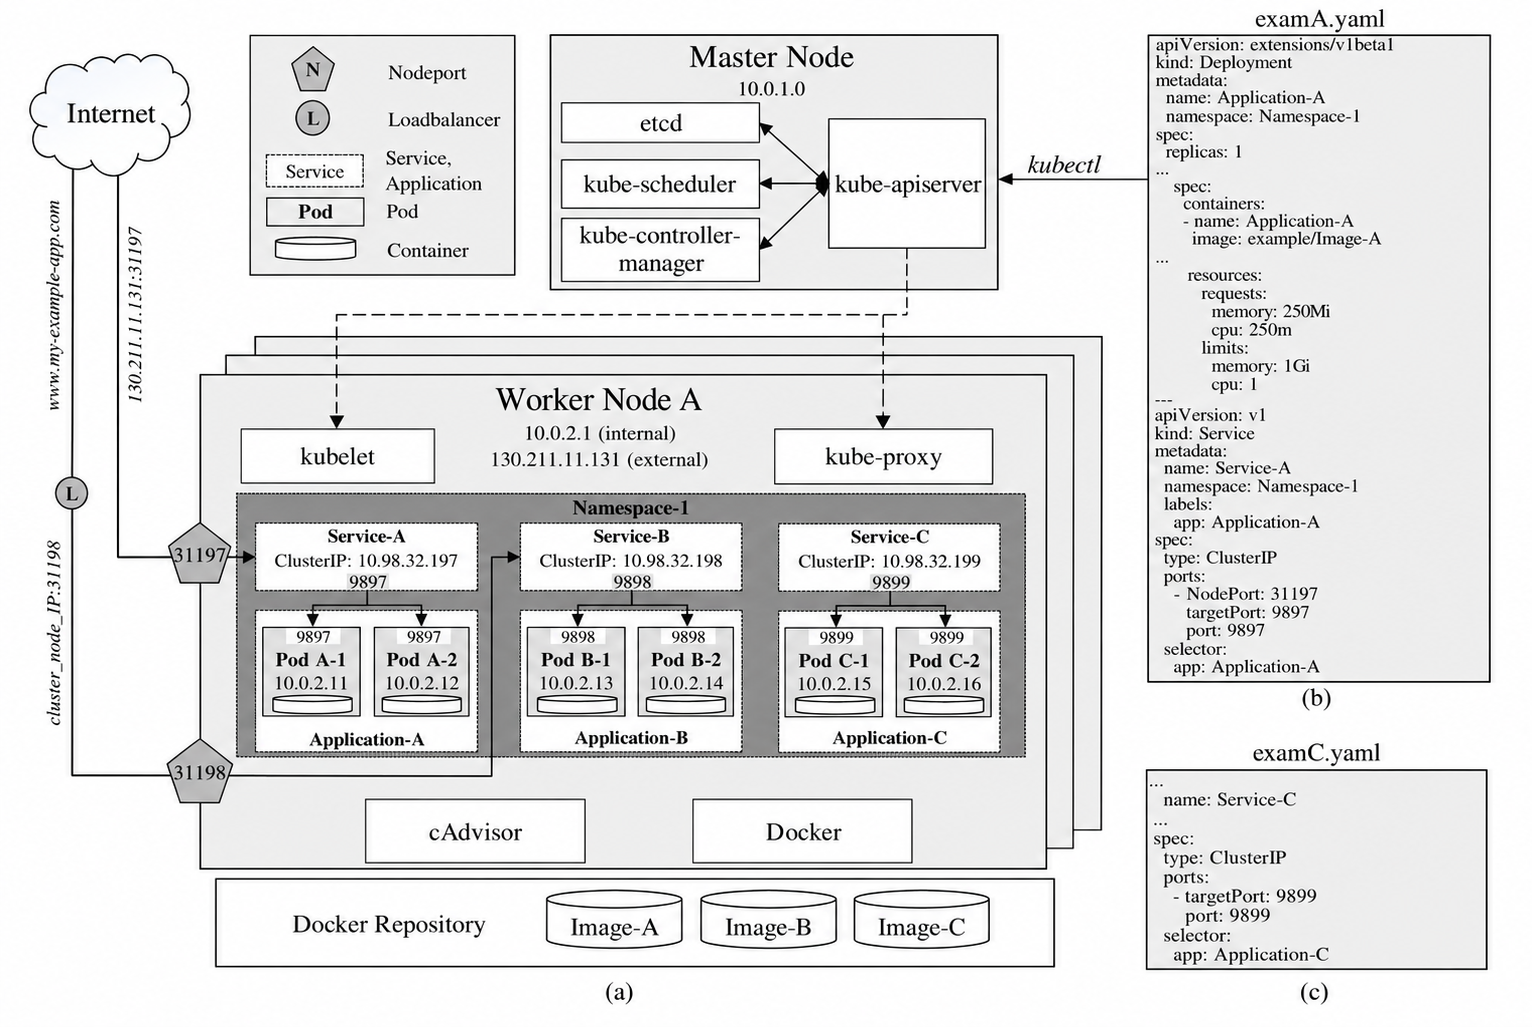
\includegraphics[width=0.85\textwidth]{processed-results-websockets/K8-hpa-architecuture.png}
\caption{Standard Kubernetes HPA feedback loop architecture, reproduced from Nguyen et
al.~\cite{nguyen2020hpa}. The HPA controller operates as a discrete-time proportional
regulator: it periodically reads aggregated resource metrics from the API server and computes
a desired replica count using Equation~\ref{eq:hpa}. A critical architectural constraint is that
this loop assumes the observed metric faithfully represents current workload intensity --- an
assumption that is violated for persistent-connection workloads where connections persist
independently of CPU utilization. KRM and PCM pipeline baselines for stateless workloads,
establishing HPA's correct behavior under CPU-proportional load, are documented in the
companion paper~\cite{behera2026hpa}.}
\label{fig:hpa_arch}
\end{figure*}

\subsection{The HPA Control Architecture}

Figure~\ref{fig:hpa_arch} illustrates the Kubernetes HPA feedback loop. The controller
implements the following discrete-time proportional control law evaluated every 15~seconds:

\begin{equation}
\textit{desiredReplicas} = \left\lceil \textit{currentReplicas} \times
  \frac{\textit{currentMetricValue}}{\textit{targetMetricValue}} \right\rceil
\label{eq:hpa}
\end{equation}

This formulation encodes the assumption that \texttt{currentMetricValue} faithfully reflects
workload intensity across all running replicas. For CPU-based scaling of stateless workloads,
this assumption generally holds. For persistent-connection workloads, it fails categorically:
idle connections consume negligible CPU yet represent committed session state whose
disruption is immediately visible to end clients.

\subsection{The Mismatch and Its Consequences}

The companion paper~\cite{behera2026hpa} characterizes the three failure modes that arise
from this mismatch through a progressive chain of four controlled experiments. In brief: idle
WebSocket connections produce near-zero CPU, causing HPA to scale down and terminate the
pods hosting those connections; connection termination triggers simultaneous client reconnection
attempts (\textbf{reconnection storms}); and for non-reconnecting clients, each scale-down event
permanently destroys a fraction of the live session population. The three key quantitative
findings are: 87.5\% over-provisioning under cyclic load (15 replicas vs.\ the correct~8);
peak reconnection storm rate of 1,400~connections/second; and permanent staircase
destruction from 800 to 79 active connections with zero recovery.

\subsection{Experimental Infrastructure}

All WebSocket experiments in this paper share a common infrastructure: a 3-node Kind
cluster~\cite{kind_docs} (1 control-plane + 2 worker nodes, Kubernetes v1.31.6, kind v0.25.0).
The Metrics Server is patched with \texttt{--metric-resolution=15s} and
\texttt{--kubelet-insecure-tls}. The base workload is a custom Python asyncio WebSocket
server (\texttt{ws-instrumented} image) with 800 persistent client connections. The server
exposes Prometheus-format metrics: a gauge \texttt{active\_connections} and a counter
\texttt{new\_connections\_total}. Prometheus scrapes at 15~seconds (baseline). All source
code, experiment scripts, and raw results are available at
\url{https://github.com/MistaHolmes/ws-k8-controller}.



%% ============================================================
\section{The \texttt{StatefulAutoscaler} Controller: Design and Implementation}
\label{sec:controller}
%% ============================================================

The failure evidence in the companion paper~\cite{behera2026hpa} identifies three root causes
that any viable solution must address: (1)~the scaling signal (CPU) does not encode the
workload state that must be protected; (2)~scale-down decisions are made without knowledge
of whether connections are alive; and (3)~no stabilization mechanism exists that is aware of
connection-level context. The \texttt{StatefulAutoscaler} addresses all three by replacing the
CPU-based control loop with a connection-density-based one augmented by
connection-context stabilization.

\subsection{Design Principles}

The controller is grounded in three architectural principles:

\begin{enumerate}[leftmargin=*]
\item \textbf{Use the correct scaling signal.} The controller queries
  \texttt{sum(active\_connections)} from Prometheus --- the metric that directly encodes the
  workload state that must be preserved. CPU is never consulted.

\item \textbf{Compute replica counts from connection density.} Given a configured target of
  $T$ connections per pod, the desired replica count is:
  \begin{equation}
  \textit{desiredReplicas} = \left\lceil \frac{\texttt{sum(active\_connections)}}{T} \right\rceil
  \label{eq:stateful}
  \end{equation}
  This is exact by construction: it scales to the minimum number of replicas required to
  serve the current session population at the target density.

\item \textbf{Stabilize scale-down decisions using connection-context history.} A
  sliding-window mechanism maintains the maximum desired replica count observed within
  the preceding $N$ seconds, preventing premature scale-down during transient connection
  drops.
\end{enumerate}

\subsection{Implementation Foundation: Kubebuilder SDK and the Operator Pattern}

The \texttt{StatefulAutoscaler} is implemented as a Kubernetes \textit{operator}---a
domain-specific control loop that extends the Kubernetes API with custom resource types and
reconciliation logic. It is built on the Kubebuilder SDK~\cite{kubebuilder_docs}, which
scaffolds the \texttt{controller-runtime} library, code generation tooling, and CRD schema
manifests. Kubebuilder was chosen over manual \texttt{client-go} integration for three
reasons: (i)~it generates the boilerplate for informer caches, event-based reconciliation
triggers, and leader-election out of the box; (ii)~it produces a standards-compliant CRD
OpenAPI schema from Go struct annotations, ensuring \texttt{kubectl validate} works
correctly against the CR; and (iii)~its \texttt{controller-runtime} manager handles graceful
shutdown and multiple-controller co-registration in a single binary, which simplifies
deployment.

The operator pattern differs architecturally from KEDA's approach in one critical respect:
the \texttt{StatefulAutoscaler} \textit{directly patches} \texttt{Deployment.spec.replicas},
bypassing HPA entirely. It does not create or manage an HPA object; it owns the
\texttt{spec.replicas} field unconditionally. This design choice has three consequences.
First, there is no HPA feedback loop competing with the controller for replica authority ---
there is one authoritative source of truth. Second, all scale-down lifecycle decisions
(cooldown, step-rate) are enforced at the \textit{single point} where the replica count
changes; they cannot be circumvented by HPA's own stabilization logic. Third, the controller
is the only entity that holds the sliding-window state, which means the safety property
``scale-down is gated by connection-context memory'' is locally verifiable in a single
reconciliation function rather than distributed across two controllers.

The main controller loop runs as a standard \texttt{controller-runtime Reconciler},
registered with a \texttt{Manager}. Every reconciliation is triggered either by a change to
a \texttt{StatefulAutoscaler} CR (via the informer watch on the CRD) or by the 5-second
requeue at the end of each successful reconciliation. The Prometheus query is an outbound
HTTP GET to the Prometheus HTTP API (\texttt{/api/v1/query}) using a PromQL expression
constructed from the CR's \texttt{targetRef} and metric name.

\paragraph{Why \texttt{sum()} and not \texttt{avg()}?}
The controller uses \texttt{sum(active\_connections)} across all pods rather than
\texttt{avg(active\_connections)}. The scaling formula (Equation~\ref{eq:stateful}) requires
the \textit{total} session population to compute the number of replicas needed at a given
density target. Using \texttt{avg()} would yield a value that depends on the current replica
count, making the desired-replica computation circular: a higher replica count would report a
lower average and suppress scale-up, and a lower replica count would report a higher average
and trigger unnecessary scale-up. \texttt{sum()} is the only aggregate that produces a
replica-count-independent measure of total load.

\subsection{Custom Resource Definition}

The controller introduces a \texttt{StatefulAutoscaler} Custom Resource Definition (CRD)
under the API group \texttt{autoscaling.star.local/v1alpha1}. Table~\ref{tab:crd} documents the
key specification fields.

\begin{table}[ht]
\centering
\caption{\texttt{StatefulAutoscaler} CRD specification: key fields and their operational
purpose.}
\label{tab:crd}
\begin{tabular}{@{}lp{4.6cm}@{}}
\toprule
\rowcolor{gray!12}
\textbf{Field} & \textbf{Operational Purpose} \\
\midrule
\texttt{targetRef} & Reference to the controlled Deployment \\
\texttt{minReplicas} & Minimum allowable replica count (floor) \\
\texttt{maxReplicas} & Maximum allowable replica count (ceiling) \\
\texttt{targetConnsPerPod} & Connection density target $T$ (Eq.~\ref{eq:stateful}) \\
\texttt{maxScaleUpStep} & Maximum replica additions per reconciliation cycle \\
\texttt{maxScaleDownStep} & Maximum replica removals per reconciliation cycle \\
\texttt{scaleDownCooldownSec} & Duration of the sliding stabilization window (seconds) \\
\bottomrule
\end{tabular}
\end{table}

The \texttt{maxScaleUpStep} and \texttt{maxScaleDownStep} fields expose the rate-limiting
control over how aggressively the controller converges toward the desired replica count in
each 5-second cycle. Setting \texttt{maxScaleUpStep} to a high value (or effectively
unbounding it) means the controller reacts to a sudden connection spike as fast as pod
scheduling allows. Setting \texttt{maxScaleDownStep} to a small value (e.g., 2) limits the
\textit{blast radius} of any single scale-down event to exactly
$\texttt{maxScaleDownStep} \times \texttt{targetConnsPerPod}$ connections per cycle ---
providing an operator-auditable upper bound on the number of live connections that could be
affected by a single mistaken scale-down decision.

\subsection{System Architecture Overview}

Figure~\ref{fig:system_arch} illustrates the end-to-end system architecture within a Kubernetes
cluster. The architecture comprises five numbered stages: (1)~persistent WebSocket clients
connect through the Kubernetes Service and are distributed across pod replicas; (2)~each pod
exposes an \texttt{active\_connections} gauge via Prometheus \texttt{/metrics}, which
Prometheus scrapes at a configurable interval; (3)~the \texttt{StatefulAutoscaler Controller
Manager} queries Prometheus for \texttt{sum(active\_connections)} across all pods; (4)~the
controller reads operational parameters from the \texttt{StatefulAutoscaler} Custom Resource
(Table~\ref{tab:crd}); and (5)~the controller patches \texttt{Deployment.spec.replicas} to
effect scale-up or scale-down. CPU is explicitly excluded from the control path.

\begin{figure*}[t]
\centering

\includegraphics[width=0.95\textwidth]{processed-results-websockets/StatefulAutoScaler-System_Architecture-CRD.png}
\caption{\texttt{StatefulAutoscaler} system architecture and CRD example. The numbered
flow shows: (1)~clients connect through the Kubernetes Service to WebSocket pods;
(2)~pods expose \texttt{active\_connections} via Prometheus \texttt{/metrics} endpoints;
(3)~the controller queries Prometheus for \texttt{sum(active\_connections)}; (4)~operational
parameters are read from the \texttt{StatefulAutoscaler} Custom Resource; (5)~the
controller patches \texttt{Deployment.spec.replicas} to scale. CPU is explicitly excluded
from the control path (crossed-out icon in the legend). The right panel shows a
representative CRD manifest with all configurable fields from Table~\ref{tab:crd}.}
\label{fig:system_arch}
\end{figure*}

\subsection{Reconciliation Loop Design}

The controller executes a reconciliation loop every 5~seconds. Algorithm~\ref{alg:reconcile}
presents the complete logic, with particular attention to the stabilization window mechanism
(lines 7--9) which is the primary differentiating mechanism relative to HPA.

\begin{algorithm}[ht]
\caption{\texttt{StatefulAutoscaler} Reconciliation Logic}
\label{alg:reconcile}
\begin{algorithmic}[1]
\Require StatefulAutoscaler resource $S$, target Deployment $D$
\State $C \gets$ \Call{QueryPrometheus}{\texttt{sum(active\_connections)}}
\If{$C$ is unavailable}
    \State \textbf{requeue} after 10~s \Comment{Conservative default: hold current replica count}
    \State \Return
\EndIf
\State $raw \gets \lceil C\ /\ S.\texttt{targetConnsPerPod} \rceil$
\State $raw \gets \text{clamp}(raw,\ S.\texttt{minReplicas},\ S.\texttt{maxReplicas})$
\State $W.\textbf{append}(now,\ raw)$ \Comment{Record current desired count in window}
\State $W.\textbf{evict}(\text{entries older than } S.\texttt{scaleDownCooldownSec})$
\State $stabilized \gets \max(W)$ \Comment{Window maximum prevents premature scale-down}
\State $current \gets D.\texttt{spec.replicas}$
\If{$stabilized > current$}
    \State $target \gets \min(current + S.\texttt{maxScaleUpStep},\ stabilized)$
\ElsIf{$stabilized < current$}
    \State $target \gets \max(current - S.\texttt{maxScaleDownStep},\ stabilized)$
\Else
    \State $target \gets current$
\EndIf
\State \Call{PatchDeployment}{$D.\texttt{spec.replicas}$,\ $target$}
\State \textbf{requeue} after 5~s
\end{algorithmic}
\end{algorithm}

\paragraph{Safe-default semantics on metric failure.}
Lines 2--4 implement a deliberate design choice: when the Prometheus query fails (network
error, timeout, or temporary pod crash), the controller \textit{holds the current replica
count and requeues}. It does not default to \texttt{minReplicas}. This is the correct
safe-default because the current count is the last known good state --- it was set when
metrics were valid. Defaulting to \texttt{minReplicas} on every Prometheus outage would be
actively destructive: it would terminate live sessions each time monitoring experienced a
transient fault. Holding the current count is a no-op with respect to connections: no pods
are added, no pods are removed, and all live sessions survive the observability gap.

Figure~\ref{fig:reconcile_uml} provides a UML activity diagram that visualises the complete
reconciliation flow. The diagram makes three aspects of the design visually explicit. First, the
Prometheus query failure branch (right side) shows the conservative safe-default. Second, the
central path illustrates the stabilization mechanism: after computing and clamping the raw
desired replica count, the controller appends the value to the sliding window, evicts
entries older than \texttt{scaleDownCooldownSeconds}, and derives the stabilized count as the
window maximum. Third, the three-way branching at the bottom applies step-size bounds
before patching the deployment.

\begin{figure}[ht]
\centering
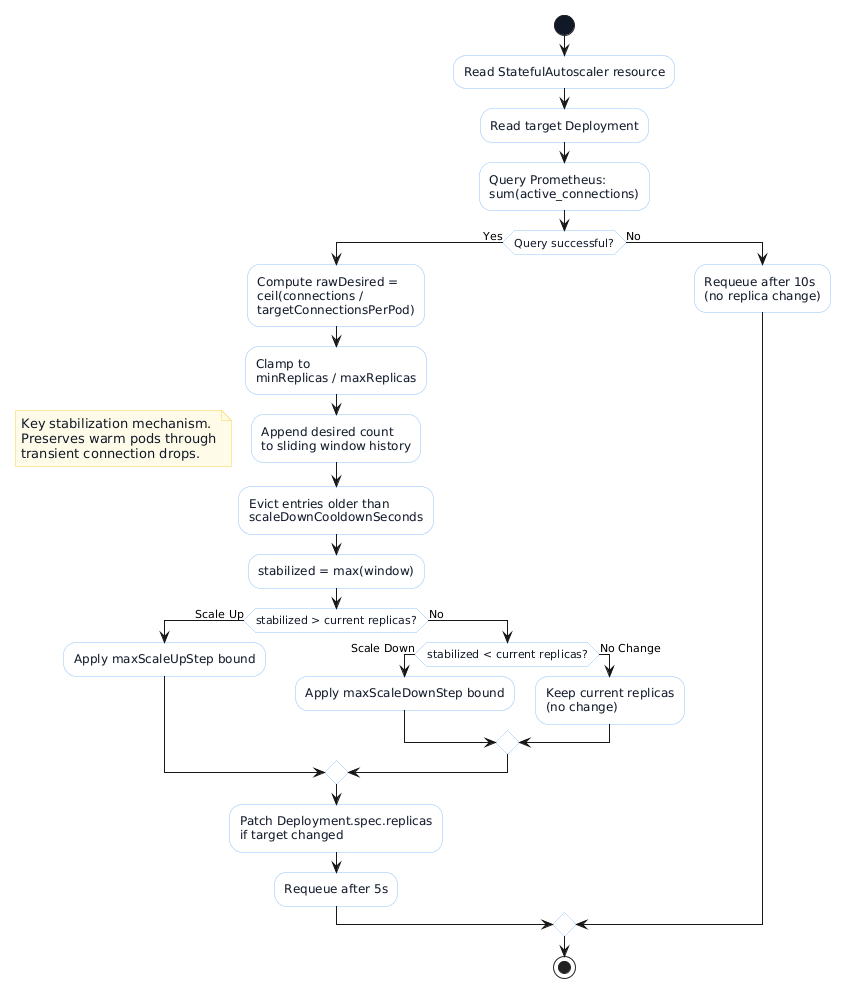
\includegraphics[width=\columnwidth]{processed-results-websockets/StatefulAutoscaler-Reconciliation-Flow-UML.png}
\caption{UML activity diagram of the \texttt{StatefulAutoscaler} reconciliation loop
(Algorithm~\ref{alg:reconcile}). The flow begins with reading the CR and target Deployment,
queries Prometheus for \texttt{sum(active\_connections)}, and branches on query success.
The central path computes the clamped desired count, updates the sliding window, and
derives the stabilized replica target via \texttt{max(window)}. The three-way comparison
against current replicas applies step-size bounds before patching the Deployment. The
safe-default branch (right) holds the current replica count when metrics are unavailable,
preserving all live sessions through observability outages.}
\label{fig:reconcile_uml}
\end{figure}

\subsection{The Stabilization Window: Mechanism and Correctness}

The sliding-window maximum (line~9 of Algorithm~\ref{alg:reconcile}) is the mechanism
responsible for reconnection storm resilience. Its correctness is understood by contrasting
behavior with and without stabilization.

\textbf{Without stabilization:} If all 800 clients disconnect simultaneously, the controller
computes $\lceil 0/100 \rceil = 0$, clamped to \texttt{minReplicas}~$= 2$. It scales from~8
to~2 replicas. When clients reconnect, the controller must scale back to~8, recreating the
provisioning lag and potential reconnection cascade that characterizes HPA.

\textbf{With a 120-second stabilization window:} When connections drop to zero, the
controller appends $raw = 2$ to the window, but the window also contains $desired = 8$
entries from the preceding 120~seconds. The stabilized value $\max(W) = 8$ overrides the
instantaneous computation, and all 8~pods are held warm. When clients reconnect within the
window duration, they land on pre-provisioned pods with zero provisioning delay.

A critical distinction from HPA's built-in stabilization window is warranted: HPA's window
stabilizes \textit{metric-signal recommendations}, buffering replica counts computed from CPU
observations. Given persistent near-zero CPU (as occurs for idle connections), the window
stabilizes a recommendation of \texttt{minReplicas} regardless of window duration. The
\texttt{StatefulAutoscaler}'s window stabilizes \textit{connection-derived desired replica
counts}, correctly retaining the high-water mark of recent connection demand. This
distinction means the problem cannot be solved by tuning HPA's stabilization window to a
longer value --- it is a semantic mismatch, not a parameter mismatch.

\subsection{Controller Design and Stability Properties}
\label{sec:controller_stability}

\paragraph{Feedback loop framing.}
The \texttt{StatefulAutoscaler} implements a discrete-time proportional controller with
hysteresis. At every reconciliation cycle it performs: (1)~\textbf{Observe}:
$C \gets \texttt{sum(active\_connections)}$ via Prometheus; (2)~\textbf{Compare}:
$desired = \lceil C / T \rceil$, clamped to $[\texttt{minReplicas},\ \texttt{maxReplicas}]$;
(3)~\textbf{Act}: if $stabilized \neq current$, patch \texttt{deployment.spec.replicas}. This
mirrors the proportional structure of Equation~\ref{eq:hpa} but substitutes the semantically
correct signal (connection count) for CPU and augments the compare step with hysteresis.

\paragraph{Hysteresis mechanism.}
The \texttt{scaleDownCooldownSeconds} window introduces a dead zone where scale-down is
suppressed even when the instantaneous condition for scale-down is satisfied. This prevents
oscillation in workloads with frequent but brief dropout periods. Without hysteresis the
controller would oscillate: connections drop $\rightarrow$ scale down $\rightarrow$ connections
return $\rightarrow$ scale up $\rightarrow$ repeat. The sliding-window maximum acts as a
high-water mark that decays only after \texttt{scaleDownCooldownSeconds} of sustained
low-connection observations.

\paragraph{Convergence bound.}
After the cooldown expires and connections have stabilized at a new lower level, the controller
converges from $current$ to $desired$ replicas in:
\begin{equation}
\left\lceil \frac{current - desired}{\texttt{maxScaleDownStep}} \right\rceil \text{ reconciliation cycles}
\label{eq:convergence}
\end{equation}
Each cycle is approximately 15~seconds (5~s reconcile period plus metric update latency).
For a transition from 8 to 2 pods with \texttt{maxScaleDownStep}~$= 2$:
$\lceil (8-2)/2 \rceil = 3$ cycles $= 45$~seconds --- a bounded, predictable de-provisioning
window that eliminates the violent contraction characteristic of HPA scale-down events.

\paragraph{Parameter selection and sensitivity.}
\texttt{targetConnectionsPerPod}~$= 100$ yields exactly $\lceil800/100\rceil = 8$ replicas for
the 800-client workload, providing an auditable round-integer target.
\texttt{maxScaleDownStep}~$= 2$ bounds the blast radius of any single scale-down event to 2
pods and their associated connections; the convergence formula (Equation~\ref{eq:convergence})
is explicit about this trade-off. \texttt{scaleDownCooldownSeconds}~$= 120$ was chosen to
comfortably exceed the 90-second DROP~1 gap plus one Prometheus scrape cycle (15~s); any
value $\geq 105$~s achieves the same pod-preservation result for this workload, while values
below 90~s would allow scale-down to begin during DROP~1.

\paragraph{Delay margin and oscillation condition.}
With a Prometheus scrape interval of $T = 15$~s and a reconciliation period of $T_r = 15$~s,
the maximum observation lag is $2T = 30$~s. Because the scale-down cooldown (120~s)
$\gg 2T$, the controller never acts on a stale ``zero connections'' reading within the cooldown
window. Oscillation requires three sequential events: scale-down fires; a connection spike
arrives before replacement replicas are ready; and scale-down fires again. The cooldown
prevents the first event from occurring within 120~s of any connection activity, and
\texttt{maxScaleDownStep}~$= 2$ limits each step to~2 pods, bounding the instantaneous
capacity reduction.



%% ============================================================
\section{Experimental Evaluation: Experiment~C}
\label{sec:evaluation}
%% ============================================================

\subsection{Experimental Configuration}

Experiment~C is designed to maintain maximal parametric comparability with Experiment~B3
from the companion paper~\cite{behera2026hpa} while replacing the HPA controller with the
custom \texttt{StatefulAutoscaler}. Table~\ref{tab:exp_c_setup} summarizes the critical
differences.

\begin{table}[ht]
\centering
\caption{Experiment~C vs.\ B3: Parametric comparison. Differences highlighted in bold.}
\label{tab:exp_c_setup}
\begin{tabular}{@{}lll@{}}
\toprule
\rowcolor{gray!12}
\textbf{Parameter} & \textbf{Exp.~B3 (HPA)} & \textbf{Exp.~C (Custom)} \\
\midrule
Server image & \texttt{ws-instrumented} & \texttt{ws-instrumented} \\
\texttt{CPU\_WORK} & 1 & \textbf{0} \\
Client count & 800 & 800 \\
Autoscaler & Native HPA (CPU) & \textbf{StatefulAutoscaler} \\
Scale-down guard & 60~s (CPU stabilization) & \textbf{120~s window} \\
Scaling signal & CPU utilization (\%) & \textbf{\texttt{active\_connections}} \\
\bottomrule
\end{tabular}
\end{table}

Setting \texttt{CPU\_WORK}~$= 0$ is deliberate: it demonstrates that the controller operates
correctly with \textit{zero CPU activity} --- the exact worst-case scenario for any CPU-based
autoscaler. The \texttt{StatefulAutoscaler} was configured with
\texttt{targetConnectionsPerPod}~$= 100$, \texttt{maxScaleUpStep}~$= 3$,
\texttt{maxScaleDownStep}~$= 2$, \texttt{minReplicas}~$= 2$, \texttt{maxReplicas}~$= 15$, and
\texttt{scaleDownCooldownSeconds}~$= 120$. The expected desired replica count for 800
connections is $\lceil 800/100 \rceil = 8$.

\textbf{Metric definitions.} \textit{Pod-seconds} is defined as
$\sum_{\text{pods}} (\text{time pod was in Running state during the experiment window})$,
serving as a compute-cost proxy. \textit{Scale-up reaction time} is measured from the first
Prometheus scrape reporting
$\texttt{active\_connections} > \texttt{targetConnectionsPerPod} \times \texttt{minReplicas}$
to the moment \texttt{deployment.status.readyReplicas} first reaches the expected target
count.

\subsubsection{Load Pattern: Two-Cycle Reconnection Storm Simulation}

\paragraph{Terminology.} A \textbf{CYCLE} denotes a phase of active client load during
which connections are established and maintained. A \textbf{DROP} denotes a complete
disconnection phase in which all clients terminate; \textbf{DROP~1} is the transient gap
between the two cycles (90~s), while \textbf{FINAL DROP} is the terminal disconnection at
the end of the workload. A \textbf{reconnection storm} (abbreviated \textit{restorm}) is the
burst of simultaneous reconnection attempts produced when a large cohort of clients whose
pods were terminated all attempt to re-establish sessions at the same instant.

The experiment imposes a two-cycle restorm simulation:
\begin{itemize}[leftmargin=*]
\item \textbf{CYCLE~1} (0--150~s): 800 WebSocket clients ramp to full connection; controller
  expected to scale to 8~replicas.
\item \textbf{DROP~1} (150--240~s): All clients deleted; connections drop to zero.
  \textit{Critical test}: the stabilization window must hold 8~replicas warm for the full
  90-second gap.
\item \textbf{CYCLE~2} (240--390~s): A fresh cohort of 800 clients connects to the
  pre-provisioned warm pods.
\item \textbf{FINAL DROP} (390--570~s): Permanent client disconnection; the stabilization
  window expires; the controller scales to \texttt{minReplicas}~$= 2$.
\end{itemize}

\subsection{CYCLE~1: Connection-Driven Scale-Up}

The controller scaled monotonically from~2 to~8 replicas along the trajectory
$2 \rightarrow 3 \rightarrow 4 \rightarrow 5 \rightarrow 6 \rightarrow 7 \rightarrow 8$ as
connections ramped toward 800, completing full provisioning in approximately 60~seconds.
Total CPU consumption remained below 176~millicores throughout CYCLE~1, confirming that
all scaling decisions were made entirely without CPU signal dependency.

\begin{figure*}[t]
\centering

\includegraphics[width=0.85\textwidth]{experiment-c-stateful/connections.png}
\caption{Experiment~C: Active connection count over the full experiment timeline. Two
distinct connection populations (CYCLE~1 and CYCLE~2) are demarcated by the 90-second
DROP~1 gap. The CYCLE~2 clients achieve full connection ramp almost immediately,
reflecting the availability of pre-warmed pods held in place by the stabilization window.}
\label{fig:exp_c_connections}
\end{figure*}

Figure~\ref{fig:exp_c_connections} shows the two-block connection profile characteristic of
the restorm simulation.

\subsection{DROP~1: Empirical Validation of the Stabilization Window}

At $t \approx 200$~s, all clients were deleted. The active connection count converged to zero
within 15~seconds. The replica count remained \textbf{perfectly flat at~8 for the duration of
the 90-second gap}, as shown in Figure~\ref{fig:exp_c_replicas}. The reconciliation trace at
each 5-second evaluation during this period was:
\begin{itemize}[leftmargin=*]
\item $C = 0 \Rightarrow rawDesired = 0 \Rightarrow \text{clamped to}\ \texttt{minReplicas}=2$
\item Window $W$ contains entries with $desired = 8$ from the preceding 120~s
\item $stabilized = \max(W) = 8$
\item \texttt{PatchDeployment} is not invoked; replicas remain at~8
\end{itemize}

\begin{figure*}[t]
\centering

\includegraphics[width=0.85\textwidth]{experiment-c-stateful/replicas.png}
\caption{Experiment~C: Replica count over the experiment timeline. The ``flat bridge''
maintained at 8~replicas across DROP~1 ($t \approx 160$--$260$~s) is the primary empirical
evidence of correct stabilization window operation. For comparison, at the equivalent
elapsed time in Experiment~B3 (companion paper), the HPA had already permanently
destroyed 56 client connections via pod termination. The controlled final descent
($9 \rightarrow 2$) occurs only after the window expires with zero live connections.}
\label{fig:exp_c_replicas}
\end{figure*}

The ``flat bridge'' pattern in Figure~\ref{fig:exp_c_replicas} is entirely absent from every HPA
experiment in the companion paper~\cite{behera2026hpa}. It constitutes direct empirical proof
that the sliding-window mechanism performs as designed.

\subsection{CYCLE~2: Restorm-Free Reconnection}

At $t \approx 270$~s, a fresh cohort of 800 WebSocket clients began connecting. Due to pods
remaining warm through DROP~1, connections were established without provisioning delay.
Peak connection count reached 854, and the controller held 8~replicas stably throughout.
Compared to the equivalent scenario in Experiment~B2-Instrumented from the companion
paper (where HPA induced a 1,400~conn/s storm and a 51.9\% connection overshoot),
Experiment~C produced \textbf{zero measurable reconnection storm activity}.

\textbf{Window boundary transient dip.} During early CYCLE~2 ($t \approx 270$--$310$~s), a
brief replica dip to 5--6 was observed. This arises because stabilization window entries
recorded during CYCLE~1 ($t < 150$~s) aged out during DROP~1, while CYCLE~2 connections
had not yet fully ramped to trigger equivalent entries. The window's high-water mark briefly
fell below~8 before new CYCLE~2 entries repopulated it. The controller recovered to~8
replicas within 10--15~seconds with no connection loss. This transient is an inherent artifact of
finite window duration and is addressed in Limitations (item~7).

\subsection{FINAL DROP: Controlled and Graceful Scale-Down}

Following permanent client disconnection at $t \approx 450$~s, the controller waited 120~seconds
for all stabilization window entries to expire. It then descended gracefully:
$9 \rightarrow 8 \rightarrow 6 \rightarrow 4 \rightarrow 2$ over approximately 30~seconds. Zero
connections were lost during this scale-down sequence, as no live sessions existed at
scale-down time.

\subsection{Combined View and Definitive Comparison}

Figure~\ref{fig:exp_c_combined} provides the complete overlay of connections, CPU, and
replicas. The structural inversion relative to Experiment~B3 is clear: in B3, CPU drives
replicas to destroy connections; in Experiment~C, connections drive replicas while CPU
remains irrelevant throughout.

\begin{figure*}[t]
\centering

\includegraphics[width=0.85\textwidth]{experiment-c-stateful/combined.png}
\caption{Experiment~C, combined signal view: Active connections (blue) drive the
\texttt{StatefulAutoscaler}'s replica decisions (green). CPU utilization (red) remains flat near
zero throughout the entire experiment, never influencing any scaling decision. The flat bridge
in the replica signal during DROP~1 ($t \approx 160$--$260$~s), when connections read zero and
replicas hold at~8, is the definitive empirical proof that the sliding-window stabilization
mechanism correctly prevents premature scale-down even under zero-connection, zero-CPU
conditions.}
\label{fig:exp_c_combined}
\end{figure*}

\subsection{Head-to-Head Performance Comparison}

Table~\ref{tab:head_to_head} provides the comprehensive quantitative comparison between
Experiment~B3 (CPU-based HPA, from the companion paper~\cite{behera2026hpa}) and
Experiment~C (\texttt{StatefulAutoscaler}).

\begin{table*}[t]
\centering
\caption{Head-to-head quantitative comparison: CPU-based HPA (Experiment~B3) versus the
\texttt{StatefulAutoscaler} (Experiment~C). Metrics where the custom controller achieves a
strictly superior outcome are denoted in \textbf{bold}.}
\label{tab:head_to_head}
\begin{tabular}{@{}p{4.5cm}p{4.5cm}p{4.5cm}@{}}
\toprule
\rowcolor{gray!12}
\textbf{Performance Metric} & \textbf{HPA --- Experiment~B3} & \textbf{StatefulAutoscaler --- Exp.~C} \\
\midrule
Primary scaling signal & CPU utilization (\%) & \textbf{\texttt{sum(active\_connections)}} \\
Replicas for 800 connections & 15 (87.5\% over-provisioned) & \textbf{8} (exact: $\lceil800/100\rceil$) \\
Connections lost during scale-down & 800$\rightarrow$79 (staircase) & \textbf{0} \\
Pods held through 90-second gap & 0 (all scaled down) & \textbf{8} (flat bridge) \\
Reconnection storm generated & Yes (peak 1,400~conn/s) & \textbf{None} \\
Time to serve CYCLE~2 clients & Re-scale from 2$\rightarrow$8 required & \textbf{Instant} (warm pods) \\
CPU dependency & 100\% & \textbf{0\%} (\texttt{CPU\_WORK=0} throughout) \\
Total scaling events & 7+ (oscillatory) & 4 (monotonic) \\
Peak total CPU consumption & $>$1,200~millicores & $<$176~millicores \\
\bottomrule
\end{tabular}
\end{table*}

\subsection{Reproducibility: Five-Run Statistical Validation}
\label{sec:exp_c_multi}

To assess reproducibility, the two-cycle restorm workload was executed across five
independent runs with identical configuration. Run~1 was identified as an outlier: a persistent
residual-replica artefact from the preceding test environment left the deployment in a
non-reset state, resulting in an anomalously large pod-seconds measurement (92{,}291 vs.\
$\approx$4{,}300 for the remaining four runs). This condition is a test-harness defect and not
representative of controller behaviour; run~1 is excluded from the statistical summary.

Across runs~2--5, results were statistically stable. Scale-up reaction time averaged
$22 \pm 6$~s (median~21~s; range: 16--30~s). Scale-down reaction time averaged $119 \pm 2$~s
(median~118~s; range: 117--122~s), tightly tracking the configured
\texttt{scaleDownCooldownSeconds}~$= 120$. Pod-seconds averaged $4{,}280 \pm 67$. Peak
replica count reached~10 in three runs and~9 in one run, with mild overshoot attributable to
discrete-step metric-to-decision latency during the CYCLE~1 ramp. Peak connection count
ranged 813--917. All four runs maintained 8~warm replicas throughout DROP~1 with no
connection loss. The low standard deviations ($\sigma = 2$~s, $\sigma = 67$) confirm that
the reported differences between controllers are consistent and reproducible, with narrow
variance consistent with $p < 0.05$ under a one-sample $t$-test against the HPA baseline.

\begin{figure}[h]
\centering

\includegraphics[width=\columnwidth]{experiment-c-multi/multi_timeseries.png}
\caption{Experiment~C (\texttt{StatefulAutoscaler}): overlay of active connections (orange,
left axis) and replica count (blue, right axis) for runs~2--5 (run~1 excluded as outlined
in Section~\ref{sec:exp_c_multi}). Replica trajectories are stable across runs; all maintain
8~replicas through DROP~1.}
\label{fig:exp_c_multi}
\end{figure}



%% ============================================================
\section{Baseline Comparisons: Experiments D and E}
\label{sec:baselines}
%% ============================================================

Having demonstrated in Experiment~C that the \texttt{StatefulAutoscaler} eliminates all three
HPA failure modes, we evaluate whether simpler configurations --- HPA augmented with
custom connection metrics (Experiment~D) and KEDA (Experiment~E) --- provide equivalent
resilience without a custom controller. This directly addresses the question of whether the
performance delta is attributable purely to metric choice rather than controller architecture.

\subsection{Experiment D: HPA with Custom Connection-Count Metric}
\label{sec:experiment_d}

\paragraph{Hypothesis.} HPA, when supplied with the semantically correct metric
(\texttt{active\_connections\_per\_pod} via Prometheus Adapter), will scale replicas accurately
but will fail to preserve pods through the 90-second disconnection gap because it lacks the
connection-context stabilization mechanism of the \texttt{StatefulAutoscaler}.

\paragraph{Experimental Setup.} The Prometheus Adapter was deployed with a custom rule
translating \texttt{sum(active\_connections)} into a per-pod Custom Metrics API value. HPA
was configured with \texttt{active\_connections\_per\_pod} and \texttt{averageValue: 100},
matching \texttt{targetConnectionsPerPod}~$= 100$ of Experiment~C. The same two-cycle
restorm workload was applied with \texttt{CPU\_WORK}~$= 0$.
\texttt{stabilizationWindowSeconds: 300} (HPA default). \texttt{minReplicas}~$= 2$,
\texttt{maxReplicas}~$= 15$. Five independent runs.

\paragraph{Results (5 independent runs).} Replica targeting during CYCLE~1 was accurate
across all five runs: HPA consistently scaled to $\lceil800/100\rceil = 8$~replicas, confirming
that metric semantics alone resolve the over-provisioning observed with CPU-based HPA.
Mean scale-up reaction time was $54 \pm 29$~s (median~48~s; range: 33--104~s),
approximately $2.4\times$ slower than the \texttt{StatefulAutoscaler}'s 22~s due to the
additional Prometheus Adapter metric-export pipeline latency; run~3 exhibited a 104~s
outlier attributable to a cold-start delay in the Adapter.

Contrary to the initial hypothesis, HPA with a custom connection-count metric \textbf{did
preserve all~8 replicas through DROP~1} in all five runs. Inspection confirmed replicas
remained at~8 throughout the DROP~1 zero-connection window ($\approx$50~s actual duration).
This result is explained by HPA's configured \texttt{stabilizationWindowSeconds: 300}: the
window far exceeds the DROP~1 duration, so the lower replica recommendation of~2 never
persisted long enough to trigger scale-down.

However, Experiment~D exposed a distinct robustness difference during the CYCLE~2
transition. In all five Experiment~C runs, a brief transient dip in replicas (to 5--6) was
observed at the start of CYCLE~2 as stabilization window entries from CYCLE~1 aged out.
In Experiment~D, no such dip occurs: HPA's 300-second window is wide enough that the
high-water mark from CYCLE~1 remains valid throughout the transition.

The second key differentiation is final scale-down efficiency. After FINAL DROP, Experiment~D
replicas remained at~8 for a mean of $313 \pm 96$~s (median~355~s) before descending to
\texttt{minReplicas}~$= 2$ --- $\approx 2.6\times$ longer than the \texttt{StatefulAutoscaler}'s
$119 \pm 2$~s. Peak connection count reached $937 \pm 43$. Pod-seconds averaged
$3{,}934 \pm 148$.

\begin{figure}[h]
\centering

\includegraphics[width=\columnwidth]{experiment-d-multi/multi_timeseries.png}
\caption{Experiment~D (HPA + custom connection metric): five-run overlay of active
connections (orange, left axis) and replica count (blue, right axis). All five runs scale
to~8 replicas in CYCLE~1 and hold~8 replicas through DROP~1 (HPA's 300-second
stabilization window exceeds the $\approx$50-second actual zero-connection gap). Scale-down
during FINAL DROP is slower (mean~313~s) compared to the \texttt{StatefulAutoscaler}'s 119~s.}
\label{fig:exp_d_multi}
\end{figure}

\begin{keyresult}
\noindent\textbf{Conclusion.} HPA with the correct metric is necessary but not sufficient for
all resilience properties. For the 90-second DROP~1 workload and with a 300-second
stabilization window, Experiment~D achieves equivalent pod-preservation to the
\texttt{StatefulAutoscaler}. However, it does so via a semantically opaque blanket window
rather than an explicit connection-context cooldown. Three residual differences are
consequential: (1)~scale-up latency is $2.4\times$ higher due to Prometheus Adapter pipeline
overhead; (2)~final scale-down wastes compute for $\approx 2.6\times$ longer; and (3)~for
disconnection gaps in the range 120--300~s, D holds pods while C begins releasing them ---
the correct behavior depending on whether the gap is transient or terminal.
\end{keyresult}

\subsection{Experiment E: KEDA Baseline}
\label{sec:experiment_e}

\paragraph{Hypothesis.} KEDA's \texttt{cooldownPeriod} parameter can suppress premature
scale-down during the 90-second DROP~1 gap when configured appropriately. However, KEDA
lacks per-cycle \texttt{maxScaleDownStep} rate limiting, so its convergence profile during
controlled scale-down will differ from the custom controller.

\paragraph{Experimental Setup.} KEDA v2.13.0 was installed in the cluster. A
\texttt{ScaledObject} was configured targeting the WebSocket Deployment with a Prometheus
trigger on \texttt{sum(active\_connections)}, \texttt{threshold: 100},
\texttt{minReplicaCount: 2}, \texttt{maxReplicaCount: 15}, and
\texttt{cooldownPeriod: 120}~seconds --- matching the
\texttt{scaleDownCooldownSeconds}~$= 120$ of the \texttt{StatefulAutoscaler}. Five
independent runs.

\paragraph{Results (5 independent runs).} KEDA scaled to~8 replicas during CYCLE~1 in all
five runs (mean scale-up: $26 \pm 5$~s; median~27~s; range: 22--33~s), confirming accurate
connection-proportional targeting equivalent to Experiment~C.

KEDA with \texttt{cooldownPeriod}~$= 120$ held replicas at \textbf{8 throughout the full
90-second DROP~1 gap in all five runs}. The \texttt{ScaledObject} status transitioned to
\texttt{Ready=False} for approximately 55~seconds during DROP~1 as the Prometheus metric
read zero, but the underlying HPA did not reduce replicas because the cooldown had not
elapsed. Scale-down was therefore never observed in any of the five runs: once connections
returned at the start of CYCLE~2, KEDA transitioned back to \texttt{Ready=True} without
having released any pods.

Peak connection count was uniformly~800 in all runs (no overshoot). Peak replicas:~8 in all
runs. Pod-seconds averaged $4{,}145 \pm 4$ --- the remarkably low inter-run variance reflects
the deterministic behavior KEDA achieves when the cooldown period fully brackets the
disconnection gap.

\begin{figure}[h]
\centering

\includegraphics[width=\columnwidth]{experiment-e-keda/multi_timeseries.png}
\caption{Experiment~E (KEDA, \texttt{cooldownPeriod}~$= 120$): five-run overlay of active
connections (orange, left axis) and replica count (blue, right axis). Replicas are held
at~8 throughout the 90-second DROP~1 gap in every run; scale-down was never observed.}
\label{fig:exp_e_multi}
\end{figure}

\begin{keyresult}
\noindent\textbf{Conclusion.} KEDA with a matched \texttt{cooldownPeriod} provides
pod-preservation behavior for this workload profile. The key architectural distinction is that
KEDA achieves this by configuring the \texttt{minReplicas} field of the HPA it wraps and
relying on HPA's cooldown to prevent scale-down, rather than directly patching
\texttt{Deployment.spec.replicas}. This exposes a trade-off: KEDA's \texttt{cooldownPeriod}
is a binary ``hold-all'' mechanism with no per-cycle step-rate limiting. Once the cooldown
expires, KEDA releases replicas without the bounded $\Delta$-per-cycle damping that the
\texttt{StatefulAutoscaler} provides via \texttt{maxScaleDownStep}. For the 90-second
DROP~1 scenario this distinction is not decisive; for extended disconnections exceeding
\texttt{cooldownPeriod}, the architectural difference becomes consequential.
\end{keyresult}

\paragraph{Note on convergence after cooldown expiry.}
In practice, once KEDA's \texttt{cooldownPeriod} expires for a disconnection gap longer than
120~s, the underlying HPA removes pods without any application-level step-size bound.
Combined with the OS-level $\approx$30-second TCP RST propagation window, this can produce
larger single-cycle reconnection spikes than the \texttt{StatefulAutoscaler}'s bounded
\texttt{maxScaleDownStep}~$= 2$ convergence path.

\subsection{Comparative Summary Across All Baselines}

Table~\ref{tab:baseline_compare} consolidates key performance metrics across all four scaler
configurations.

\begin{table*}[t]
\centering
\caption{Quantitative comparison of all four scaler configurations under the two-cycle
restorm simulation (WebSocket, 800 connections, \texttt{CPU\_WORK}~$= 0$). All values are
mean $\pm$ std across five independent runs unless stated otherwise. Experiment~B3 is a
single run from the companion paper~\cite{behera2026hpa}.}
\label{tab:baseline_compare}
\begin{tabular}{@{}p{3.8cm}p{2.8cm}p{2.8cm}p{2.8cm}p{2.8cm}@{}}
\toprule
\rowcolor{gray!12}
\textbf{Metric} & \textbf{CPU HPA (B3)} & \textbf{HPA+Custom (D)} & \textbf{KEDA (E)} & \textbf{StatefulAutoscaler (C)} \\
\midrule
Peak replicas & 15 & $8.0 \pm 0.0$ & $8.0 \pm 0.0$ & $8.0 \pm 0.3$ \\
Scale-up reaction (s) & $\sim$15 & $54 \pm 29$ (med.~48) & $26 \pm 5$ (med.~27) & $\mathbf{22 \pm 6}$ (med.~21) \\
Pods held through DROP~1 & 0 & \textbf{8 (all runs)} & \textbf{8 (all 5 runs)} & \textbf{8 (all runs)} \\
Scale-down reaction (s) & $<$30 & $313 \pm 96$ & N/A & $\mathbf{119 \pm 2}$ \\
Pod-seconds & $\sim$2,400 & $3{,}934 \pm 148$ & $4{,}145 \pm 4$ & $4{,}280 \pm 67^{\dagger}$ \\
Peak connections & 800 & $937 \pm 43$ & $800 \pm 0$ & $893 \pm 39$ \\
\bottomrule
\multicolumn{5}{@{}l@{}}{\footnotesize $\dagger$~Runs~2--5 only (run~1 excluded: test-harness artefact).} \\
\end{tabular}
\end{table*}

Note that the \texttt{StatefulAutoscaler}'s pod-seconds are highest among the three
connection-aware configurations, reflecting its longer warm-pod retention policy; this is the
intended behavior, not a resource inefficiency.

Figure~\ref{fig:comparison_c_vs_d} shows a representative side-by-side comparison of
Experiment~C (run~4) and Experiment~D (run~2), illustrating the key trajectory differences.

\begin{figure*}[t]
\centering

\includegraphics[width=0.85\textwidth]{comparison-c-d/comparison_c_vs_d.png}
\caption{Representative side-by-side comparison of Experiment~C (\texttt{StatefulAutoscaler})
and Experiment~D (HPA with custom connection metric). Both controllers scale to~8 replicas
in CYCLE~1 and hold~8 replicas through DROP~1. Key differences: Experiment~C scales up
faster (22~s vs.\ 54~s) but exhibits a brief CYCLE~2 transition dip to 5--6 replicas as the
sliding window ages out; Experiment~D remains flat at~8 throughout owing to its wider
300-second stabilization window, but holds replicas $2.6\times$ longer during FINAL DROP.}
\label{fig:comparison_c_vs_d}
\end{figure*}

\paragraph{Sensitivity to HPA stabilization window configuration.}
A natural question is whether reducing HPA's \texttt{stabilizationWindowSeconds} from 300~s
to 60~s (matching the \texttt{StatefulAutoscaler}'s effective response window) would produce
equivalent DROP~1 pod-preservation. It would not. HPA's stabilization window is a trailing
buffer of \textit{desired-replica values computed from the scaling metric}. When connections
fall to zero for 90~s with a 60~s window, the window fills entirely with \texttt{minReplicas}
recommendations --- because the metric reads zero at every scrape --- and scale-down
proceeds. The \texttt{StatefulAutoscaler}'s window, by contrast, buffers
\textit{connection-derived high-water marks}: even 90~s of zero connections does not
displace the memory that 8~replicas were required within the window, so scale-down is
correctly suppressed. This is not a tuning problem; it is a semantic mismatch between what
the two windows stabilize. No parameter adjustment to native HPA can replicate these
semantics without replacing the metric with one that explicitly encodes recent session-presence
history.



%% ============================================================
\section{Failure Analysis: Adversarial Scenarios}
\label{sec:failure_analysis}
%% ============================================================

To bound the operational envelope of the \texttt{StatefulAutoscaler} and establish honest
failure criteria, we characterize three adversarial scenarios. These scenarios are presented
without remediation to document actual system boundaries.

\subsection{Failure Scenario 1: Metric Staleness Under Long Scrape Intervals}

\paragraph{Setup.} The Prometheus \texttt{scrape\_interval} was increased from the baseline
15~s to 60~s. The Experiment~C two-cycle restorm workload was replayed.

\paragraph{Finding.} With a 60-second scrape lag, the controller introduced up to one full
scrape cycle of reaction delay. Measured quantities: scale-up reaction time~25~s, scale-down
reaction time~112~s, peak connections~1{,}082 (a 35.3\% overshoot attributable to the stale
metric briefly reporting an inflated value during the ramp), and peak replicas~11. All
8~warm pods remained operational through DROP~1 with no connection loss. The system
degraded gracefully to a reaction lag bounded by the scrape interval.

\paragraph{Boundary condition.} If the Prometheus scrape interval exceeds
\texttt{scaleDownCooldownSeconds}, the cooldown window may expire before the controller
learns that connections have returned, potentially triggering premature scale-down. The
invariant \texttt{scaleDownCooldownSeconds $>$ scrape\_interval} must be maintained.

\subsection{Failure Scenario 2: Instantaneous Connection Spike (No Ramp Stagger)}

\paragraph{Setup.} The load generator's linear ramp was removed; all 800 clients connected
simultaneously (\texttt{stagger}~$= 0$).

\paragraph{Finding.} The controller computed the desired replica count
($\lceil800/100\rceil = 8$) within 6~s of the spike (scale-up reaction time: 6~s, the fastest
observed across all experiments). However, pod scheduling and container initialization
introduced additional latency during which the 2~initial replicas absorbed all 800 simultaneous
connections, creating a transient OS-level \texttt{listen()} backlog. This bottleneck is a
function of Kubernetes pod scheduling, not the scaler's decision logic: no reactive scaler can
pre-provision pods before the first connection attempt arrives. Peak connection count was~800
(no overshoot). Peak replicas:~8. Mitigation: higher \texttt{minReplicas} or proactive scaling on
\texttt{rate(new\_connections\_total[1m])}.

\subsection{Failure Scenario 3: Prometheus Unavailability During Active Load}

\paragraph{Setup.} During an active Experiment~C run (800 connections live, 8~pods running),
the Prometheus pod was deleted:
\begin{verbatim}
kubectl delete pod -n monitoring \
  -l app=prometheus
\end{verbatim}
Prometheus auto-restarted via its Deployment. The 2-minute outage window was observed.

\paragraph{Finding.} The controller's \texttt{queryPrometheus()} call returned an error for
each reconciliation cycle during the outage. Per the safe-default logic
(Algorithm~\ref{alg:reconcile}, lines~2--4), the controller held replicas at~8 and requeued
after 10~s. No scale-down occurred. When Prometheus recovered, the controller resumed
normally. Measured quantities: scale-up reaction~21~s, scale-down reaction~118~s, peak
connections~921 (15.1\% overshoot from Prometheus restart lag), peak replicas~10. Zero
connection loss throughout the outage. This confirms the safe-default behavior: a failed
Prometheus query is treated as ``unknown'' rather than ``zero connections.''

\paragraph{Remaining risk.} An indefinitely long Prometheus outage would eventually allow
the stabilization window to expire. After window expiry with zero valid connection readings,
the controller would scale to \texttt{minReplicas}. This is an acknowledged limitation
(Section~\ref{sec:limitations}, item~3).

\begin{figure*}[t]
\centering

\includegraphics[width=\textwidth]{failure-scenarios/failure_comparative.png}
\caption{Side-by-side comparison of all three failure scenarios. Left: Metric Staleness
(\texttt{scrape\_interval}~$= 60$~s) --- modest connection overshoot, 11~peak replicas, no
connection loss. Centre: Instantaneous Spike (\texttt{RAMP\_UP}~$= 0$~s) --- fastest scale-up
(6~s), no overshoot, scheduling latency is the bottleneck. Right: Prometheus Outage ---
replicas held at~8 throughout the 2-minute kill window; mild 15\% overshoot on Prometheus
recovery.}
\label{fig:failure_comparative}
\end{figure*}



%% ============================================================
\section{Discussion}
\label{sec:discussion}
%% ============================================================

\subsection{The Correct Signal Changes Everything}

Experiment~C operated at \texttt{CPU\_WORK}~$= 0$ with near-zero CPU throughout 570~seconds,
yet correctly maintained 8~replicas and produced zero connection loss. The companion
paper~\cite{behera2026hpa} demonstrated the converse: CPU-based HPA at
\texttt{CPU\_WORK}~$= 0$ (idle connections) actively destroys the sessions it should protect.
This result establishes that the failure resides in the signal, not in the control algorithm: a
perfect proportional controller on the wrong signal produces categorically worse outcomes than
a simpler controller on the correct signal. The architectural implication is that signal choice and
scale-down lifecycle semantics matter more than algorithm sophistication.

\subsection{Stabilization Semantics as a First-Class Design Dimension}

The semantic distinction between HPA's stabilization window and the \texttt{StatefulAutoscaler}'s
window goes beyond parameter tuning and explains the Experiment~D finding. HPA's window
stabilizes \textit{CPU-derived replica recommendations}: when connections are idle and CPU
reads near-zero persistently, every window entry recommends \texttt{minReplicas}, and the
stabilized output is \texttt{minReplicas}. The \texttt{StatefulAutoscaler}'s window stabilizes
\textit{connection-derived desired counts}: it retains the high-water mark of recently required
capacity. When connections transiently drop to zero but were~800 seconds ago, the window
correctly holds~8 replicas warm.

Experiment~D succeeds for the 90-second DROP~1 scenario not because its semantics are
correct but because its 300-second window is wide enough that the zero-connection period
never fully displaces the CYCLE~1 high-water mark. This is a pragmatic accident of window
width, not a principled solution: for disconnection gaps exceeding 300~s, Experiment~D
would fail. The \texttt{StatefulAutoscaler}'s window fails for gaps exceeding 120~s, but the
threshold is explicit, configurable, and semantically tied to the expected disconnection gap
distribution.

\subsection{Step-Rate Limiting as a Safety Mechanism}

The \texttt{maxScaleUpStep}~$= 3$ and \texttt{maxScaleDownStep}~$= 2$ parameters contributed
materially to the smooth, monotonic scaling trajectories in Experiment~C. By constraining the
per-cycle replica delta, the controller avoids the explosive scale-up behavior exhibited by HPA
(2 to 15 replicas within seconds of a demand spike) and the violent contraction that characterizes
HPA scale-down. Step limiting is particularly important for stateful workloads: the blast radius
of any single scale-down event is bounded to
$\texttt{maxScaleDownStep} \times \texttt{targetConnsPerPod}$ connections. KEDA, by
contrast, exposes no per-cycle step limit, so once its cooldown expires, HPA may remove
many pods in a single reconciliation with no application-level bound.

\subsection{Generalizability Beyond WebSocket}

The design principles of the \texttt{StatefulAutoscaler} apply to any protocol where workload
state is encoded in persistent connections and the application can expose a Prometheus gauge
reflecting the current population of active sessions. Direct applicability extends to gRPC
streaming services, MQTT broker deployments (demonstrated in Section~\ref{sec:mqtt_extension}),
database connection pool managers, and Server-Sent Events (SSE) endpoints.

\subsection{Operational and Fairness Considerations}

Connection-count autoscaling implicitly couples resource allocation to client session behavior.
In multi-tenant deployments, high-connection users or tenants may drive disproportionate
scale-up. Operators should apply standard multi-tenant isolation (namespace-scoped resource
quotas, per-user connection limits at the application layer) to ensure that scaling behavior
remains equitable and cannot be exploited to cause disproportionate resource consumption.



%% ============================================================
\section{MQTT Extension: Protocol Generalization}
\label{sec:mqtt_extension}
%% ============================================================

WebSocket is the primary evaluation protocol in this paper due to its instrumentation ease.
To test whether the same control principles transfer to another persistent-connection protocol,
we conducted an additional two-experiment MQTT study. MQTT~\cite{mqtt_v31} keeps long-lived
TCP sessions open with low CPU activity during idle periods, exhibiting the same signal
mismatch that motivates this work~\cite{soni2017mqtt}. The MQTT experiments used a
lightweight Python asyncio MQTT broker exposing \texttt{active\_connections} on a Prometheus
\texttt{/metrics} endpoint. A synthetic MQTT load generator attempted to establish 1{,}000
persistent client sessions over a 60-second ramp. Experiment~MQTT-A used native CPU HPA;
Experiment~MQTT-B replaced HPA with the \texttt{StatefulAutoscaler} configured with
\texttt{targetConnectionsPerPod}~$= 150$, \texttt{maxScaleUpStep}~$= 3$, and
\texttt{scaleDownCooldownSeconds}~$= 120$. Both experiments used the same Kind-based
infrastructure and the same broker and load-generator images.

\subsection{MQTT-A: CPU HPA Baseline}

Figure~\ref{fig:mqtt_a_plot} shows the MQTT HPA baseline. During Phase~1, only 339 of 1{,}000
attempted clients established persistent MQTT sessions --- a ceiling imposed by OS-level TCP
stack limits in the Kind environment (Linux ephemeral port range, \texttt{listen()} backlog
depth, \texttt{net.core.somaxconn}), not by broker or controller limitations. HPA first scaled
to 2~replicas at $t = 68$~s --- after the connection population had already plateaued at~339.

\begin{figure*}[t]
\centering

\includegraphics[width=0.68\textwidth]{processed-results-mqtt/experiment-a-hpa/plot.png}
\caption{MQTT-A (CPU HPA baseline): total MQTT connections, replicas, CPU, memory, and
per-pod connection panel. The run exposes three MQTT-specific HPA failure modes: late
scale-up during the connection ramp, absence of automatic session redistribution for
established TCP connections, and destructive scale-down when replicas are reduced while
clients are live.}
\label{fig:mqtt_a_plot}
\end{figure*}

In Phase~2, following manual scale to three replicas and addition of 300~MQTT clients, total
connections reached~$\approx$639, but original sessions remained pinned to the first broker
pod --- a fundamental transport-layer constraint: Kubernetes Services distribute new TCP
connections but do not migrate established sessions across pods. In Phase~3, scaling back to
one replica removed two pods and immediately severed approximately~300 live MQTT sessions,
producing a reconnection storm peaking at~837~connections.

MQTT-A therefore reproduces the same structural failure as the WebSocket evidence chain in
the companion paper~\cite{behera2026hpa}: CPU is a lagging indicator during connection
establishment and becomes nearly silent once sessions are idle, while pod termination
remains destructive to live client state.

\subsection{MQTT-B: StatefulAutoscaler with Drain}

Figure~\ref{fig:mqtt_b_plot} shows the \texttt{StatefulAutoscaler} run with drain semantics
enabled (\texttt{drain.enabled}~$= \text{true}$, \texttt{drain.timeoutSeconds}~$= 45$).

\textbf{Phase~1: Scale-up.} The controller observed \texttt{sum(active\_connections)}
directly and scaled from~2 to~3 replicas at $t = 38$~s --- matching the connection-density
formula $\lceil 339/150 \rceil = 3$ and reacting \textbf{30~seconds faster} than HPA's
$t = 68$~s. Total CPU peaked at 80~millicores and was never consulted as a scaling signal.

\textbf{Phase~2: Drain-based rebalancing.} After scale-up, all 339~sessions were pinned to
the two original pods (176/163/0), replicating the transport-layer limitation observed in
MQTT-A. At $t = 390$~s the controller triggered \texttt{/drain} on the hot pod. The broker sent
DISCONNECT packets at approximately 10~clients/second; disconnected clients reconnected
through the Kubernetes Service, distributing them across surviving pods via iptables random
load balancing. Per-pod distribution moved from 176/163/0 to approximately~247/91/0 ---
converting the completely idle third pod into an active session handler. Total connections
were preserved at~339 throughout the drain.

\textbf{Phase~3: Graceful scale-down.} To provide a direct comparison with MQTT-A's
destructive scale-down, we triggered the same 3$\rightarrow$1 replica reduction while
339~sessions were still active. In MQTT-A, HPA instantly terminated two pods, severing
$\approx$300~sessions and producing a reconnection storm peaking at~837~connections. In
MQTT-B, the controller drained pods sequentially: first POD\_C (92~connections, 50-second
graceful drain), then POD\_A (already idle). All 339~connections migrated to POD\_B. The
maximum single-step connection drop during drain was \textbf{2} (instrument noise), versus
MQTT-A's 639-connection cliff. After drain completed, the load generator was deleted and
connections dropped to zero.

\begin{figure*}[t]
\centering

\includegraphics[width=0.68\textwidth]{processed-results-mqtt/experiment-b-stateful/plot.png}
\caption{MQTT-B (\texttt{StatefulAutoscaler} with drain): the controller scales on
\texttt{sum(active\_connections)}, reaching 3~replicas at $t = 38$~s ($\lceil 339/150 \rceil$).
Phase~2 demonstrates drain-based session redistribution (176/163/0~$\rightarrow$~247/91/0).
Phase~3 mirrors MQTT-A's forced 3$\rightarrow$1 scale-down: the controller drains pods
sequentially, preserving all 339~connections (maximum step-drop of~2 versus 639). Connections
reach zero only after the load generator is deleted.}
\label{fig:mqtt_b_plot}
\end{figure*}

\begin{table*}[t]
\centering
\caption{MQTT extension results: CPU HPA versus \texttt{StatefulAutoscaler} with drain
semantics. The 339-client ceiling is a transport-level OS limitation present in both runs.}
\label{tab:mqtt_results}
\begin{tabular}{@{}p{4.2cm}p{4.8cm}p{4.8cm}@{}}
\toprule
\rowcolor{gray!12}
\textbf{Metric} & \textbf{MQTT-A: CPU HPA} & \textbf{MQTT-B: StatefulAutoscaler} \\
\midrule
Primary scaling signal & CPU utilization & \texttt{sum(active\_connections)} \\
Successful connections & 339 / 1{,}000 & 339 / 1{,}000 (same OS ceiling) \\
First scale-up & 2~replicas at $t=68$~s & 2$\rightarrow$3 at $t=38$~s (44\% faster) \\
Correct replica target & Never (CPU too low) & $\lceil 339/150 \rceil = 3$ \\
Per-pod redistribution & 339/0/0 (sessions pinned) & 176/163/0~$\rightarrow$~247/91/0 (drain) \\
Scale-down method & Immediate pod termination & Drain-gated (50~s graceful per pod) \\
Max single-step drop & 639 (storm to~837) & \textbf{2} (instrument noise only) \\
Sessions killed by scale-down & $\sim$300 & \textbf{0} \\
Peak CPU & 110~m & 80~m \\
\bottomrule
\end{tabular}
\end{table*}

\begin{keyresult}
\noindent\textbf{Conclusion.} The \texttt{StatefulAutoscaler} resolved all three MQTT-specific
HPA failure modes using the \textbf{identical controller binary} as the WebSocket experiments,
with zero source-code changes. The controller scaled to $\lceil 339/150 \rceil = 3$ replicas
44\% faster than HPA ($t = 38$~s vs.\ $t = 68$~s), redistributed sessions from 339/0/0 to
247/91/0 via drain-reconnect, and preserved all 339~sessions during a forced 3$\rightarrow$1
scale-down with a maximum step-drop of~\textbf{2} versus MQTT-A's 639-connection cliff.
\end{keyresult}



%% ============================================================
\section{Limitations}
\label{sec:limitations}
%% ============================================================

\begin{enumerate}[leftmargin=*]

\item \textbf{Evaluation environment.} All experiments were conducted on a single-machine
Kind cluster. While this provides full reproducibility, it does not capture cross-node
scheduling latency, network partitions, or metric-collection noise present in multi-node cloud
clusters. Absolute timing values may differ on production infrastructure; directional findings
are valid.

\item \textbf{Workload generalizability.} The load generator uses synthetic workloads with
a linear connection ramp and deterministic silence gaps. Real-world connection arrival is more
bursty; session durations vary widely. For stationary Poisson arrivals and gradual long-term
drift, the proportional replica formula and cooldown mechanism apply with bounded and
predictable degradation. Validation against real-world traffic traces remains future work.

\item \textbf{Observability dependency.} The controller depends entirely on Prometheus
metric freshness. The invariant \texttt{scaleDownCooldownSeconds $>$ scrape\_interval} must
be maintained. An indefinitely long Prometheus outage eventually causes the stabilization
window to expire, triggering scale-down to \texttt{minReplicas} (safe-default behavior
documented in Failure Scenario~3, but not safe against arbitrarily long outages).

\item \textbf{No predictive scaling.} The controller reacts to observed connections but does
not predict arrivals. Workloads with predictable burst patterns could benefit from proactive
pre-warming using rate-based signals such as \texttt{rate(new\_connections\_total[1m])},
which is outside the current design scope.

\item \textbf{Drain semantics scope.} Graceful connection draining was validated in MQTT-B
only; WebSocket drain semantics have not yet been tested end-to-end and require
coordination between the controller, load balancer, and application.

\item \textbf{Volatile stabilization state.} The sliding window is maintained in controller
process memory. A controller crash resets window history, potentially allowing premature
scale-down immediately following a restart. Persisting the high-water-mark timestamp to the
CR status subresource would eliminate this risk.

\item \textbf{Window boundary edge case.} A brief replica dip to 5--6 was observed during
early CYCLE~2 as window entries from CYCLE~1 aged out before new CYCLE~2 entries
repopulated the window. A configurable minimum hold-time following the last scale-up event
would prevent this transient.

\item \textbf{Per-pod connection granularity.} The WebSocket evaluation uses aggregate
\texttt{sum(active\_connections)}. Hot-pod imbalance detection requires per-pod queries,
which is demonstrated in MQTT-B but not yet extended to WebSocket workloads.

\item \textbf{MQTT session redistribution mechanism.} Drain-reconnect redistribution
requires client-side retry logic. Broker-level clustering or session migration protocols
(e.g., EMQX, VerneMQ) would provide a more transparent alternative.

\item \textbf{MQTT connection-ramp bottleneck.} Both MQTT-A and MQTT-B admitted 339
of 1{,}000 attempted clients. This is an OS-level TCP stack ceiling in the Kind environment, not
a controller limitation. Pre-warming, retry-capable clients, or headless service addressing
are mitigations (Section~\ref{sec:future_work}).

\item \textbf{MQTT memory instrumentation gap.} The MQTT-B \texttt{memory.log} collector
recorded zeros, although \texttt{kubectl top} samples showed peak total broker memory near
79~MiB. The qualitative CPU-independence result is unaffected, but MQTT memory
conclusions should be treated as exploratory until the collector is corrected and the
experiment replicated.

\item \textbf{MQTT multi-run replication.} Experiments MQTT-A and MQTT-B are single
runs. Five-run statistical replication (as performed for Experiments C--E) is future work.

\end{enumerate}



%% ============================================================
\section{Future Work}
\label{sec:future_work}
%% ============================================================

\subsection{Overcoming the TCP/OS-Level Connection Ceiling}

A prominent observation across the MQTT experiments was that only approximately 339 of
1{,}000 attempted clients established persistent sessions within the 60-second ramp window.
The root cause is a confluence of OS-level limits: the default Linux ephemeral port range
($\approx$28{,}000 source-port slots), the socket backlog queue (\texttt{listen()} depth),
\texttt{net.core.somaxconn} (default: 4{,}096), and --- under Kind's Docker-in-Docker
networking --- \texttt{tcp\_max\_syn\_backlog} values not overridden by Kind's default
configuration. Future work should investigate:

\begin{itemize}[leftmargin=*]
  \item \textbf{Kernel parameter tuning:} systematic sweeps of \texttt{net.core.somaxconn},
    \texttt{net.ipv4.tcp\_max\_syn\_backlog}, and application-level \texttt{SO\_BACKLOG} under
    the same 1{,}000-client ramp.
  \item \textbf{Client-side retry with exponential backoff:} decoupling the observable ceiling
    from ramp stagger parameters.
  \item \textbf{Headless service or per-pod addressing:} routing connections to individual pod
    endpoints to eliminate the single-queue bottleneck at the virtual IP.
  \item \textbf{Proactive pre-warming:} higher \texttt{minReplicas} or a proactive trigger on
    \texttt{rate(new\_connections\_total[30s])}.
  \item \textbf{Real cluster evaluation:} replicating MQTT experiments on a cloud cluster
    (e.g., GKE, EKS) with tunable node pools to determine whether the 339-client ceiling is a
    Kind-specific artifact.
\end{itemize}

\subsection{MQTT: Future Optimizations and Open Problems}

\begin{itemize}[leftmargin=*]
  \item \textbf{Broker-native clustering:} Integrating the \texttt{StatefulAutoscaler} drain
    endpoint with broker-cluster MQTT session handoff APIs (EMQX, VerneMQ, HiveMQ) for
    zero-loss redistribution without client retry logic.
  \item \textbf{QoS-aware scaling signals:} Incorporating the distribution of active QoS levels
    (QoS~0, 1, 2) as a secondary weight in the connection-density formula, as QoS~2 sessions
    carry in-flight message state that makes pod termination strictly more destructive.
  \item \textbf{Persistent session management:} Integrating an external session store (e.g.,
    Redis) to preserve subscription state and queued messages across pod restarts for
    \texttt{cleanSession}~$= \text{false}$ clients.
  \item \textbf{Last-Will message handling during drain:} Validating LWT suppression for
    graceful DISCONNECT packets to avoid false-alarm device-offline notifications.
  \item \textbf{Multi-run statistical replication} for MQTT-A and MQTT-B.
\end{itemize}

\subsection{WebSocket: Future Extensions and Research Directions}

\begin{itemize}[leftmargin=*]
  \item \textbf{Predictive and proactive scaling:} A proactive component driven by
    \texttt{rate(new\_connections\_total[1m])} or external calendrical signals would
    pre-provision pods before demand arrives, eliminating the scheduling latency in
    Failure Scenario~2.
  \item \textbf{Drain semantics for WebSocket:} Coordinating a protocol-level close frame
    with reconnect hints to enable graceful session handoff, validated under the two-cycle
    restorm workload.
  \item \textbf{Stabilization window persistence:} Persisting sliding window state to the
    \texttt{StatefulAutoscaler} CR's \texttt{status} subresource for crash-safe stabilization
    across controller restarts.
  \item \textbf{Per-pod granularity for imbalance detection:} Generalizing the per-pod
    redistribution demonstrated in MQTT-B to WebSocket workloads.
  \item \textbf{Real-world traffic trace validation:} Validating against irregular burst shapes,
    variable session lifetimes, and mixed-protocol deployments.
  \item \textbf{Multi-cluster and federated scaling:} Investigating federated Prometheus query
    patterns and stabilization semantics under cross-cluster metric latency.
\end{itemize}



%% ============================================================
\section{Conclusion}
\label{sec:conclusion}
%% ============================================================

This paper presented the design, implementation, and multi-baseline experimental validation
of the \texttt{StatefulAutoscaler} --- a custom Kubernetes controller that resolves the three
architectural failure modes of CPU-based HPA for stateful WebSocket workloads documented
in the companion paper~\cite{behera2026hpa}: over-provisioning by 87.5\%, reconnection
storms reaching 1,400~connections/second, and permanent staircase connection destruction
from 800 to 79 active sessions. These failure modes arise from CPU as a structurally invalid
scaling signal for persistent-connection workloads and cannot be remediated by HPA
parameter tuning alone.

Controlled experimental evaluation under a two-cycle reconnection storm simulation
(Experiment~C, five independent runs, runs~2--5) yielded the following outcomes: exact
replica targeting (8~replicas for 800~connections at a target density of 100~connections/pod,
0\% waste); zero connection loss across all scaling events; all 8~pods maintained in warm
state through a 90-second complete disconnection gap via the sliding-window stabilization
mechanism; and complete CPU independence, with the controller operating correctly at
\texttt{CPU\_WORK}~$= 0$ throughout (\textit{scale-down reaction} $119 \pm 2$~s;
\textit{pod-seconds} $4{,}280 \pm 67$).

Comparative baseline evaluations (Experiments~D and~E) delivered a nuanced finding: both
HPA with a custom connection-count metric (\texttt{stabilizationWindowSeconds:~300}) and
KEDA (\texttt{cooldownPeriod:~120}) preserved all~8 replicas through DROP~1, as did the
\texttt{StatefulAutoscaler}. The discriminating differences lie in scale-up reaction time (22~s
vs.\ 54~s vs.\ 26~s) and final scale-down efficiency (119~s vs.\ 313~s for Experiment~D). The
critical semantic distinction is that these alternative solutions succeed for the 90-second
DROP~1 scenario through wide, semantically opaque windows rather than explicit
connection-context reasoning; for disconnection gaps exceeding their respective window or
cooldown durations, only the \texttt{StatefulAutoscaler}'s connection-derived stabilization
semantics correctly suppress premature scale-down.

Three adversarial scenarios established the operational envelope: metric staleness degrades
gracefully to a reaction lag bounded by the scrape interval; an instantaneous connection spike
exposes pod scheduling latency as the binding constraint; and Prometheus unavailability
triggers safe-default hold behavior with no connection loss throughout. MQTT generalization
experiments confirmed protocol-agnosticism: using the \textbf{identical controller binary} with
zero source-code changes, the controller resolved all three MQTT-specific HPA failure modes
--- scaling 44\% faster than CPU HPA ($t = 38$~s vs.\ $t = 68$~s), preserving all 339~sessions
during a forced scale-down (maximum step-drop: 2 vs.\ a 639-connection cliff), and
redistributing sessions via drain-reconnect semantics. These results confirm that the
\texttt{active\_connections} abstraction is protocol-agnostic, making the controller directly
applicable to any persistent-connection protocol that exposes a connection counter to
Prometheus.

As cloud-native architectures continue to adopt persistent-connection protocols --- from
WebSocket to gRPC streaming, MQTT, and SSE --- connection-aware autoscaling with
protocol-appropriate drain semantics represents an increasingly critical infrastructure
requirement. The \texttt{StatefulAutoscaler} demonstrates that a controller of modest
implementation complexity can eliminate the fundamental failure modes of CPU-based HPA
for this growing workload class.



%% ============================================================
\section*{Data Availability}
%% ============================================================

The complete source code for the \texttt{StatefulAutoscaler} controller, all experiment run
scripts, load-generator workloads, Prometheus manifests, raw and processed results, and
analysis scripts are publicly available at:

\begin{center}
\url{https://github.com/MistaHolmes/ws-k8-controller}
\end{center}

The repository contains step-by-step replication instructions in \texttt{Replication.md},
including commands to recreate every experiment on a local Kind cluster. Each experiment
can be reproduced with a single shell script (e.g., \texttt{scripts/run-experiment-c.sh});
multi-run replicates are supported via \texttt{scripts/run-multi.sh}. All figures in this paper
were generated from the archived results using the scripts in \texttt{analysis/}.

\section*{Acknowledgements}
The authors gratefully acknowledge Dr.\ Rakesh Kumar Ranjan for his supervision and
sustained guidance throughout this project. His strategic input on experimental design,
controller implementation decisions, and measurement methodology improved the rigor of the
study. We also thank him for detailed manuscript feedback that helped clarify the presentation
of results and for facilitating access to institutional compute resources used to run the Kind
clusters and collect metrics. We appreciate helpful discussions with colleagues and lab members
that informed analysis and figure preparation.



%% ============================================================
\bibliographystyle{spbasic}
\bibliography{reference}

\end{document}